In this section we try to find a model able to explain the variable \textit{"PTS"} through regression techniques.

First of all a preliminary analysis was performed on the data to get some intuitive insights about their composition and relations.
In figure \Fig~\ref{fig:CorrMatrix} is given the correlation matrix over all the dataset.
\begin{figure}[h]
	\centering
	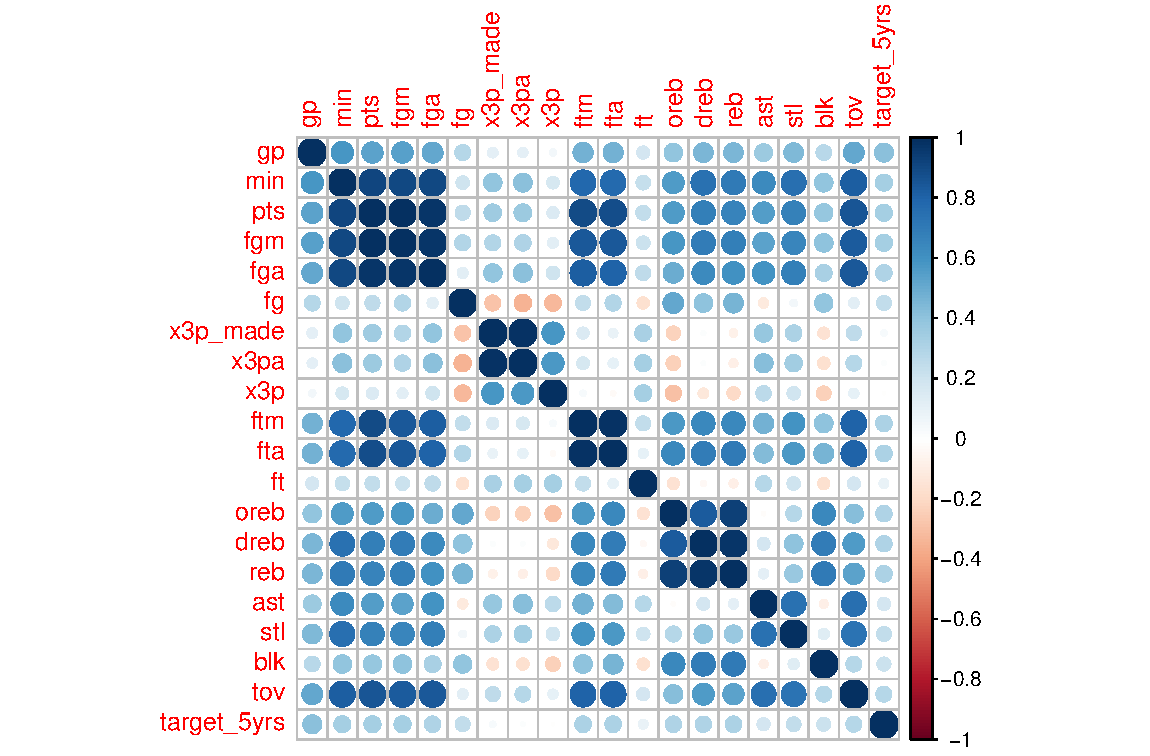
\includegraphics[width=0.5\linewidth]{ImageFiles/Regression/CorrMatrix}
	\caption{Correlation matrix.}
	\label{fig:CorrMatrix}
\end{figure}

From that matrix is possible to see that \textit{"PTS"} is strongly correlated with \textit{"MIN"}. Indeed, intuitively players who play more time has chances to gain points, and of course players who make more points will be put on the game for more time by the coach. Therefore this result is consistent with the intuition.

The other two variables strongly correlated are \textit{"FGM"} and \textit{"FGA"}, but for different reasons in this case. Actually \textit{"FGM"} tells the number of field goals made and those are the main source of points. Indeed, fitting a linear model using only \textit{"FGM"} as regressors we obtained a model with $R^2 = 0.98$. Similarly for \textit{"FGA"} since they same quantities expressed in percentage. With this remark in mind, we decided to drop both this variables because they are almost equivalent to the target, and they are not interesting for analysis purposes.

After this overview, subset selection and regularization methods were applied to select the variables to include in the model. More precisely:
\begin{itemize}
	\item Forward Stepwise Selection
	\item Backward Stepwise Selection
	\item Ridge Regression
	\item Lasso Regression
\end{itemize}

At the end we compared the four models obtained.
